%!TEX program = xelatex

\documentclass[12pt,a4paper]{article}
\usepackage{xeCJK}
\usepackage{amsmath}
\setCJKmainfont{STSongti-SC-Regular}
\usepackage{setspace}
\usepackage{caption}
\usepackage{graphicx, subfig}
\usepackage{float}
\usepackage{listings}
\usepackage{booktabs}



\begin{document} 
\title{homework3}
	\author{11611118 郭思源}  

\section{Problem 1}
\begin{lstlisting}[language=matlab]
%指数分布
set(gcf,'Units','centimeters','Position',[0 0 30 30]);
num = [100,1000,5000];
mu = 3;
for i = 1:3
sample = exprnd(mu,num(i),1);% Simulated data
x=min(sample):1:max(sample);
subplot(3,3,3*i-2)
histogram(sample,x);
title(sprintf('Exponential distribution (n=%d)', num(i)));
fprintf("i=%d",i);
[muhat,muci] = expfit(sample, 0.05)
end

%泊松分布
num = [100,1000,5000];
lam=70;
for i = 1:3
sample=poissrnd(lam,num(i),1);% Simulated data
x=min(sample):1:max(sample);
subplot(3,3,3*i-1)
histogram(sample,x);
title(sprintf('Poisson distribution (n=%d)', num(i)));
fprintf("i=%d",i);
[Lambdahat, Lambdaci]=poissfit (sample, 0.05)
end

%正态分布
num = [100,1000,5000]*2;
for i = 1:3
sample = normrnd(0,1,num(i),1);
x=min(sample):0.1:max(sample);
subplot(3,3,3*i)
histogram(sample,x);
title(sprintf('Normal distribution (n=%d)', num(i)));
fprintf("i=%d",i);
[muhat,sigmahat,muci,sigmaci]=normfit(sample, 0.05)
end
\end{lstlisting}

\begin{figure}[htbp]
\centering
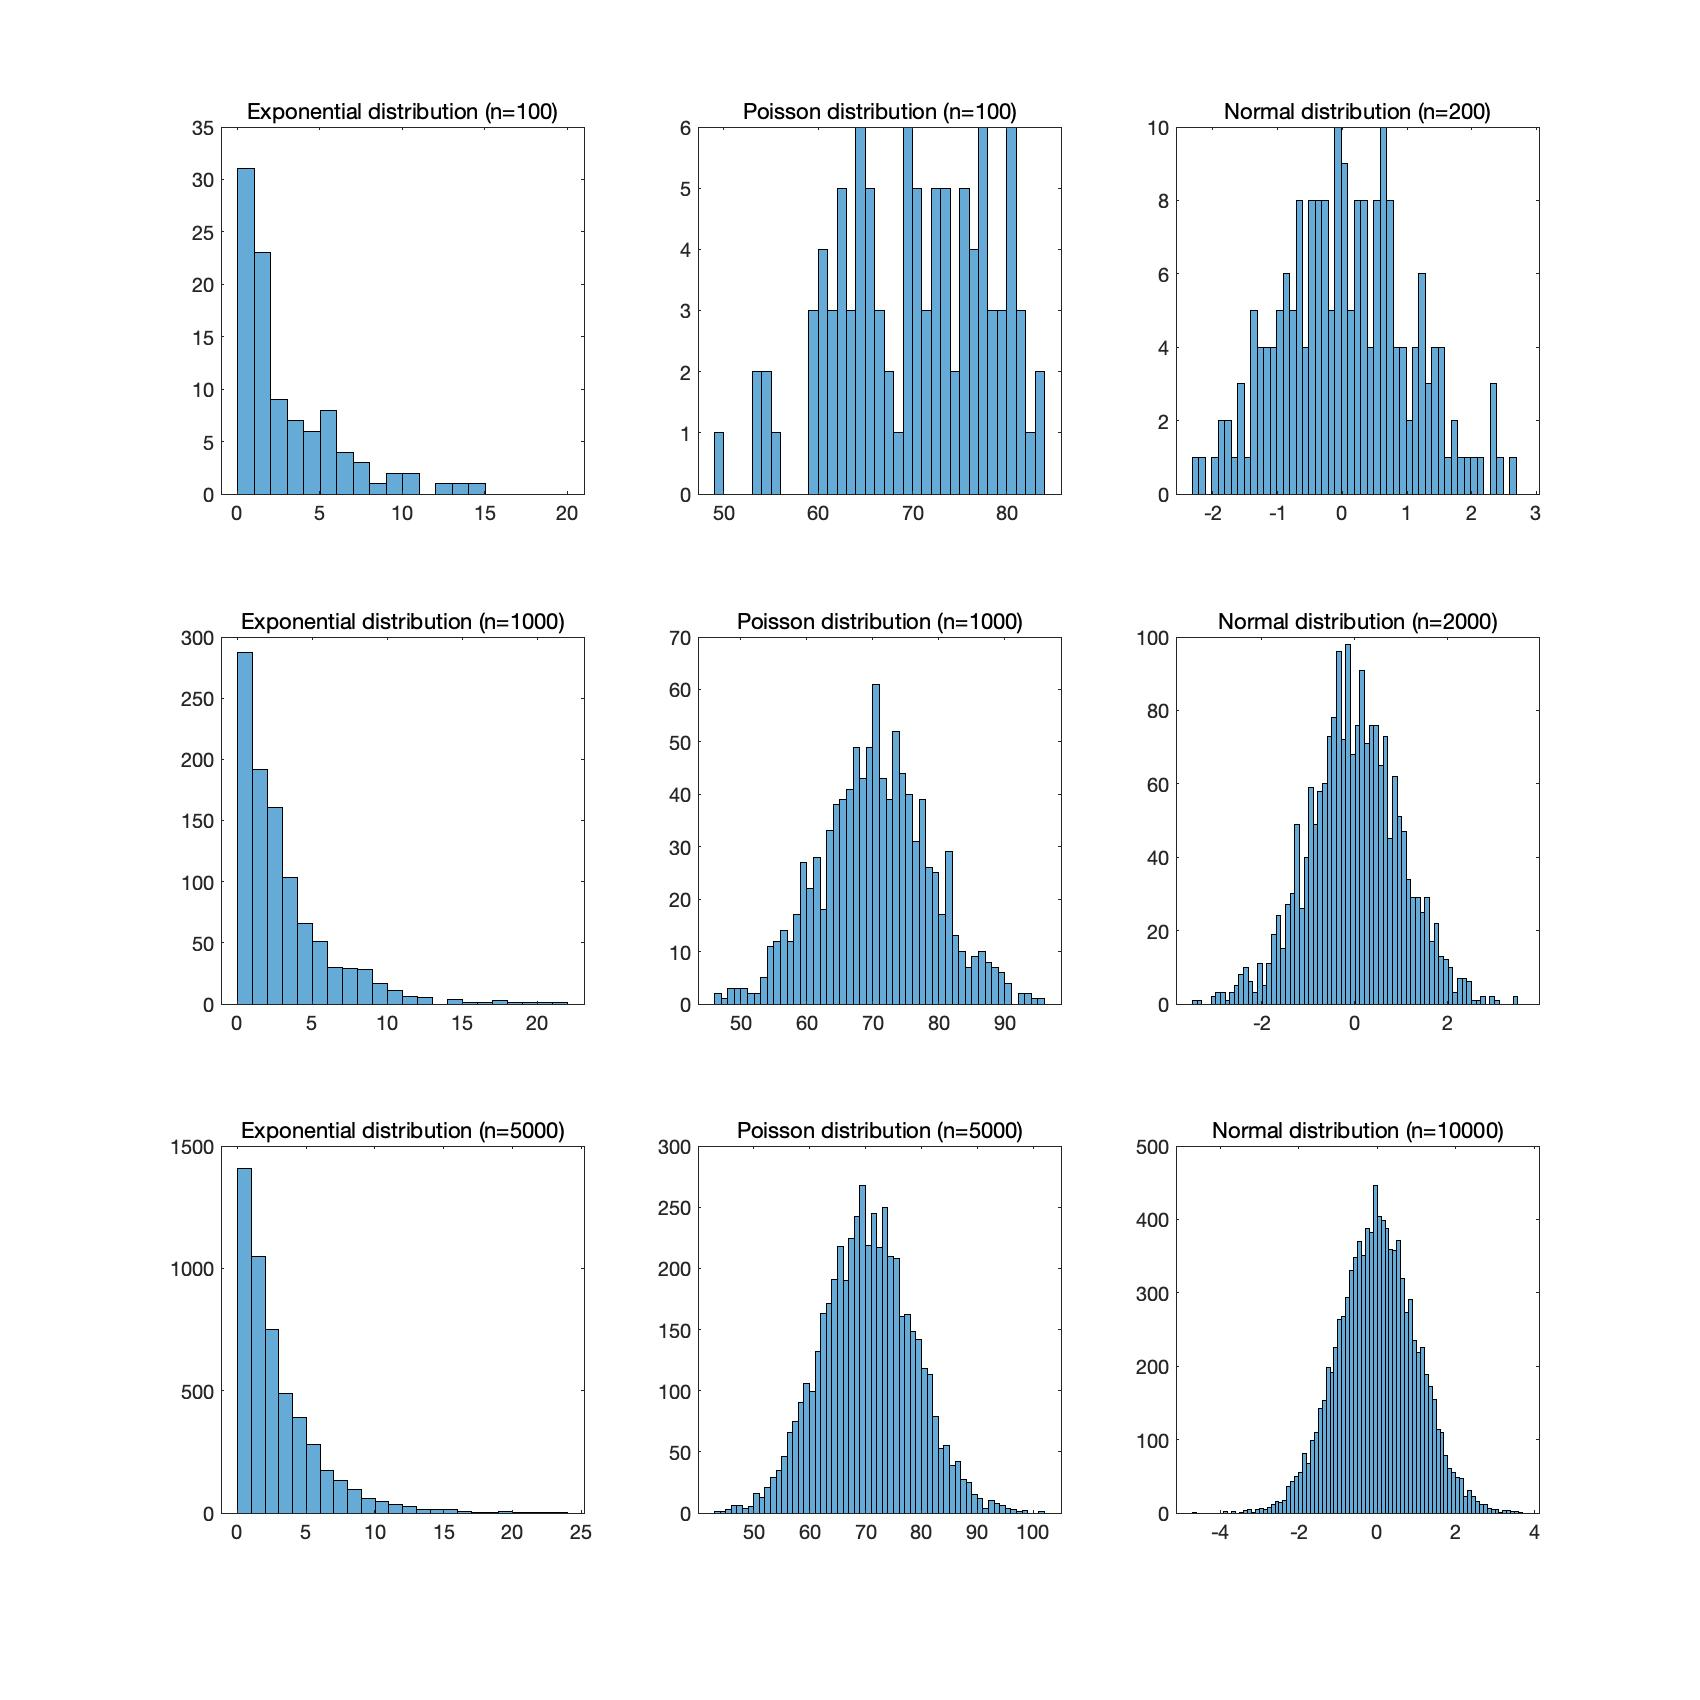
\includegraphics[bb=400 400 1300 1300,scale=.3]{figure/HW3_1.jpg}
\end{figure}

\begin{table}[htbp]
\caption{Exponential distribution confidence interval (95)\% \\ $\lambda=3$} 
\centering
\begin{tabular}{lll}
	\toprule 
	Number of samples & 
	Estimates the mean $\lambda$ & 
	Confidence intervals for the mean $\lambda$ \\ 
	\midrule 
	100 & 2.7511 & [ 2.2826, 3.3813 ] \\ 
	1000 & 3.0171 & [ 2.8385, 3.2132 ] \\
	5000 & 2.9651 & [ 2.8846, 3.0490 ] \\ 
	\bottomrule 
\end{tabular} 
\end{table}

\newpage

\begin{table}[htbp]
\caption{Poisson distribution confidence interval (95)\% \\ $\lambda=70$} 
\centering
\begin{tabular}{lll}
	\toprule 
	Number of samples & 
	Estimates the mean $\lambda$ & 
	Confidence intervals for the mean $\lambda$ \\ 
	\midrule 
	100 & 70.4200 & [ 68.7753, 72.0647 ] \\ 
	1000 & 70.2070 & [ 69.6877, 70.7263 ] \\
	5000 & 69.8896 & [ 69.6579, 70.1213 ] \\ 
	\bottomrule 
\end{tabular} 
\end{table}

\begin{table}[htbp]

\caption{Exponential distribution confidence interval (95)\% \\ 
		$\mu=0$ \\ $\sigma=1$} 
\centering

\begin{tabular}{lll}

	\toprule 
	Number of samples & 
	Estimates the mean $\mu$ & 
	Confidence intervals for the mean $\mu$ \\ 
	\midrule 
	200 & 0.0279 & [ -0.1152, 0.1710 ] \\ 
	2000 & 0.0099 & [ -0.0339, 0.0536 ] \\
	10000 & -0.0122 & [ -0.0318, 0.0074 ] \\ 
	\bottomrule 

\end{tabular} 

\begin{tabular}{lll}

	\toprule 
	Number of samples & 
	Estimates the mean $\sigma$ & 
	Confidence intervals for the mean $\sigma$ \\ 
	\midrule 
	200 & 1.0263 & [ 0.9346, 1.1381 ] \\ 
	2000 & 0.9977 & [ 0.9677, 1.0296 ] \\
	10000 & 0.9990 & [ 0.9854, 1.0131 ] \\ 
	\bottomrule 

\end{tabular} 

\end{table}


\newpage

\section{Problem 2}

\subsection{0-norm}
As we know the error 
$\left\|e\right\|_0$ = the number of ${y_i-ax_i-b\ne0}$\\
so that we choose the line y=ax+b such that the most point lie on the line.\\
so we just choose two point $(x_i,y_i)$ $(x_j,y_j)$\\

Then: \\
\begin{equation}
	\begin{aligned}
		a &= \frac{y_i-y_j}{x_i-x_j}\\
		b &= \frac{y_j x_i-x_j y_i}{x_i-x_j}\\
	\end{aligned}
\end{equation}


\subsection{1-norm}
 

As we know the error $\left\|e\right\|_1$=$\sum_{i=1}^n|y_i-ax_i-b|$\\

Error: \\
\begin{equation}
	\begin{aligned}
		\Bar{e} &= \frac{\sum_{i=1}^n|y_i-ax_i-b|}{n} \\
		e_i &= |y_i-ax_i-b|\\
	\end{aligned}
\end{equation}

So we define y$_i$$'$=$y_i-| e_i- \Bar{e} |$\\

\noindent So that we can know that those  y$_i$$'$ lie on two parallel lines. and the fit line is the middle line of those tow liens. 

So is y$_i$$'$ satisfy:\\
\begin{equation}
	\begin{aligned}
		y &= ax+b \pm \Bar{e} \\ 
	\end{aligned}
\end{equation}
 



\newpage
\subsection{2-norm}
As we know the error $\left\|e\right\|_2$=$\sum_{i=1}^n(y_i-ax_i-b)^2$\\

So : 
\begin{equation}
	\begin{aligned}
		\frac{\partial e}{\partial a} &= 0 \\
		\frac{\partial e}{\partial b} &= 0 \\\\
	\end{aligned}
\end{equation}

Then :
\begin{equation}
	\begin{aligned}
		a &= \frac{m \sum_{i=1}^n{x_i y_i}-\sum_{i=1}^n{x_i} \sum_{i=1}^n{y_i}}{m \sum_{i=1}^n{x_i^2}-(\sum_{i=1}^n{x_i})^2}\\\\
		b &= \frac{\sum_{i=1}^n{x_i^2} \sum_{i=1}^n{y_i}-\sum_{i=1}^n{x_i} m \sum_{i=1}^n{x_i y_i}}{m \sum_{i=1}^n{x_i^2}-(\sum_{i=1}^n{x_i})^2}
	\end{aligned}
\end{equation}


\subsection{$\infty$-norm}
As we know the error $\left\|e\right\|_\infty$=$\max{|y_i-ax_i-b|}$\\
Suppose when i=k,$|y_i-ax_i-b|$ is maximum\\
so that we just make the a,b to satisfy $ax_k-b=y_k$ \\
Then we will get the min $\left\|e\right\|_\infty$\\


\newpage

\section{Problem 3}
The lasso in Matlab is used for lasso or elastic net regularization for linear models. \\\\
\textbf{The syntax of the lasso function:}\\

\noindent \textbf{B = lasso(X,Y):}\\
Returns fitted least-squares regression coefficients for linear models of the predictor data X and the response y. Each column of B corresponds to a particular regularization coefficient in Lambda. By default, lasso performs lasso regularization using a geometric sequence of Lambda values.\\

\noindent \textbf{B = lasso(X,Y,Name,Value):}\\
Fits regularized regressions with additional options specified by one or more name-value pair arguments. For example, 'Alpha',0.5 sets elastic net as the regularization method, with the parameter Alpha equal to 0.5.\\

\noindent \textbf{$\textbf{[B,FitInfo]}$ = lasso($\_\_\_$):}\\
For any previous input syntax, also returns a structure containing information about the fits. It invokes a normalized regression analysis that is appropriate for additional options with specific names and values.\\

\noindent \textbf{Input: }\\\\
\textbf{X} is the numeric matrix. Each row represents one observation, and each column represents one predictor (variable).\\\\
\textbf{Y} is the numeric vector of length n, where n is the number of rows of \textbf{X}. \textbf{Y(i)} is the response to row i of \textbf{X}.\\

\noindent \textbf{ADMM algorithm:}\\\\
ADMM algorithm is used in an agrument called AbsTol which is used in the lasso to deal with tall array data.\\
ADMM is the algorithm that expands by ALM solves convex optimization problems by breaking them into smaller pieces, each of which are then easier to handle. It is aimed to make up the shortcomings of secondary punishment to make the algorithm more stable\\

\end{document}

